\documentclass[letterpaper,12pt]{article}
\usepackage{tabularx,amsmath,boxedminipage,graphicx}
\usepackage[margin=1in,letterpaper]{geometry} % this shaves off default margins which are too big
\usepackage{cite}
\usepackage[final]{hyperref} % adds hyper links inside the generated pdf file
\hypersetup{
	colorlinks=true,       % false: boxed links; true: colored links
	linkcolor=blue,          % color of internal links
	citecolor=blue,        % color of links to bibliography
	filecolor=magenta,      % color of file links
	urlcolor=blue         
}

\begin{document}
\title{EC413 Lab 6: 3-Stage 32-bit Pipelined Datapath}

\author{Austin M. Welch}
\date{\today}
\maketitle

\begin{abstract}

The main objective of this lab was to gain a better understanding of the timing that goes on
in a pipelined datapath by simulating MIPS instruction codes and tracing them through three
stages of registers. 

\end{abstract}

\section{Introduction}

 Figure~\ref{fig:top_diagram} shows the structure of the entire 32-bit pipelined datapath. Each of these six components is contained in my top module.

\begin{figure}[hb] 
        % read manual to see what [ht] means and for other possible options
        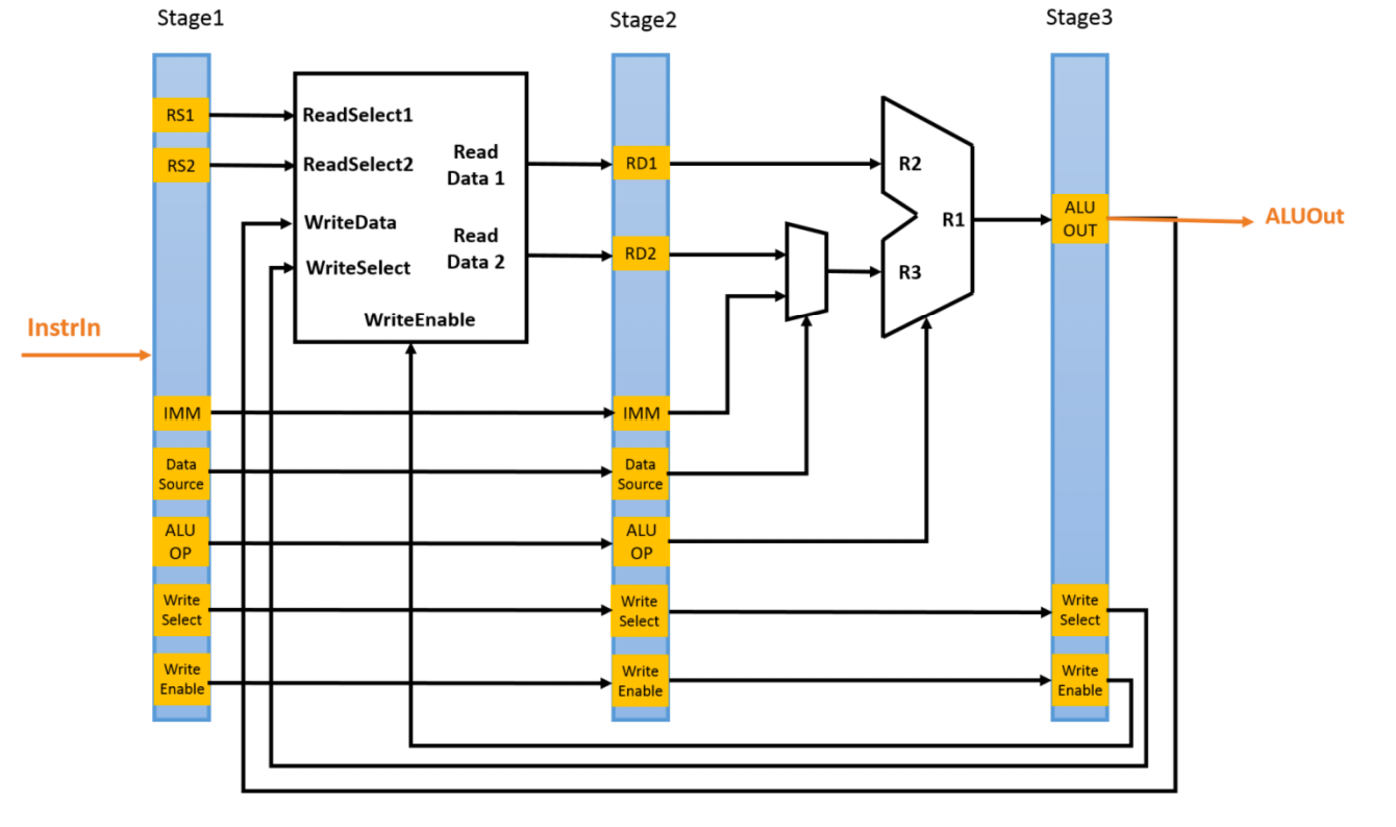
\includegraphics[width=1.0\columnwidth]{pipeline_pic}
        % note that in above ___________________^^^^^^^^^figure file name
        % the file extension is missing. LaTeX is smart enough to find
        % apropriate one (i.e. pdf, png, etc.)
        % You can add this extention yourself as it seen below
        % both notations are correct but above has more flexibility
        %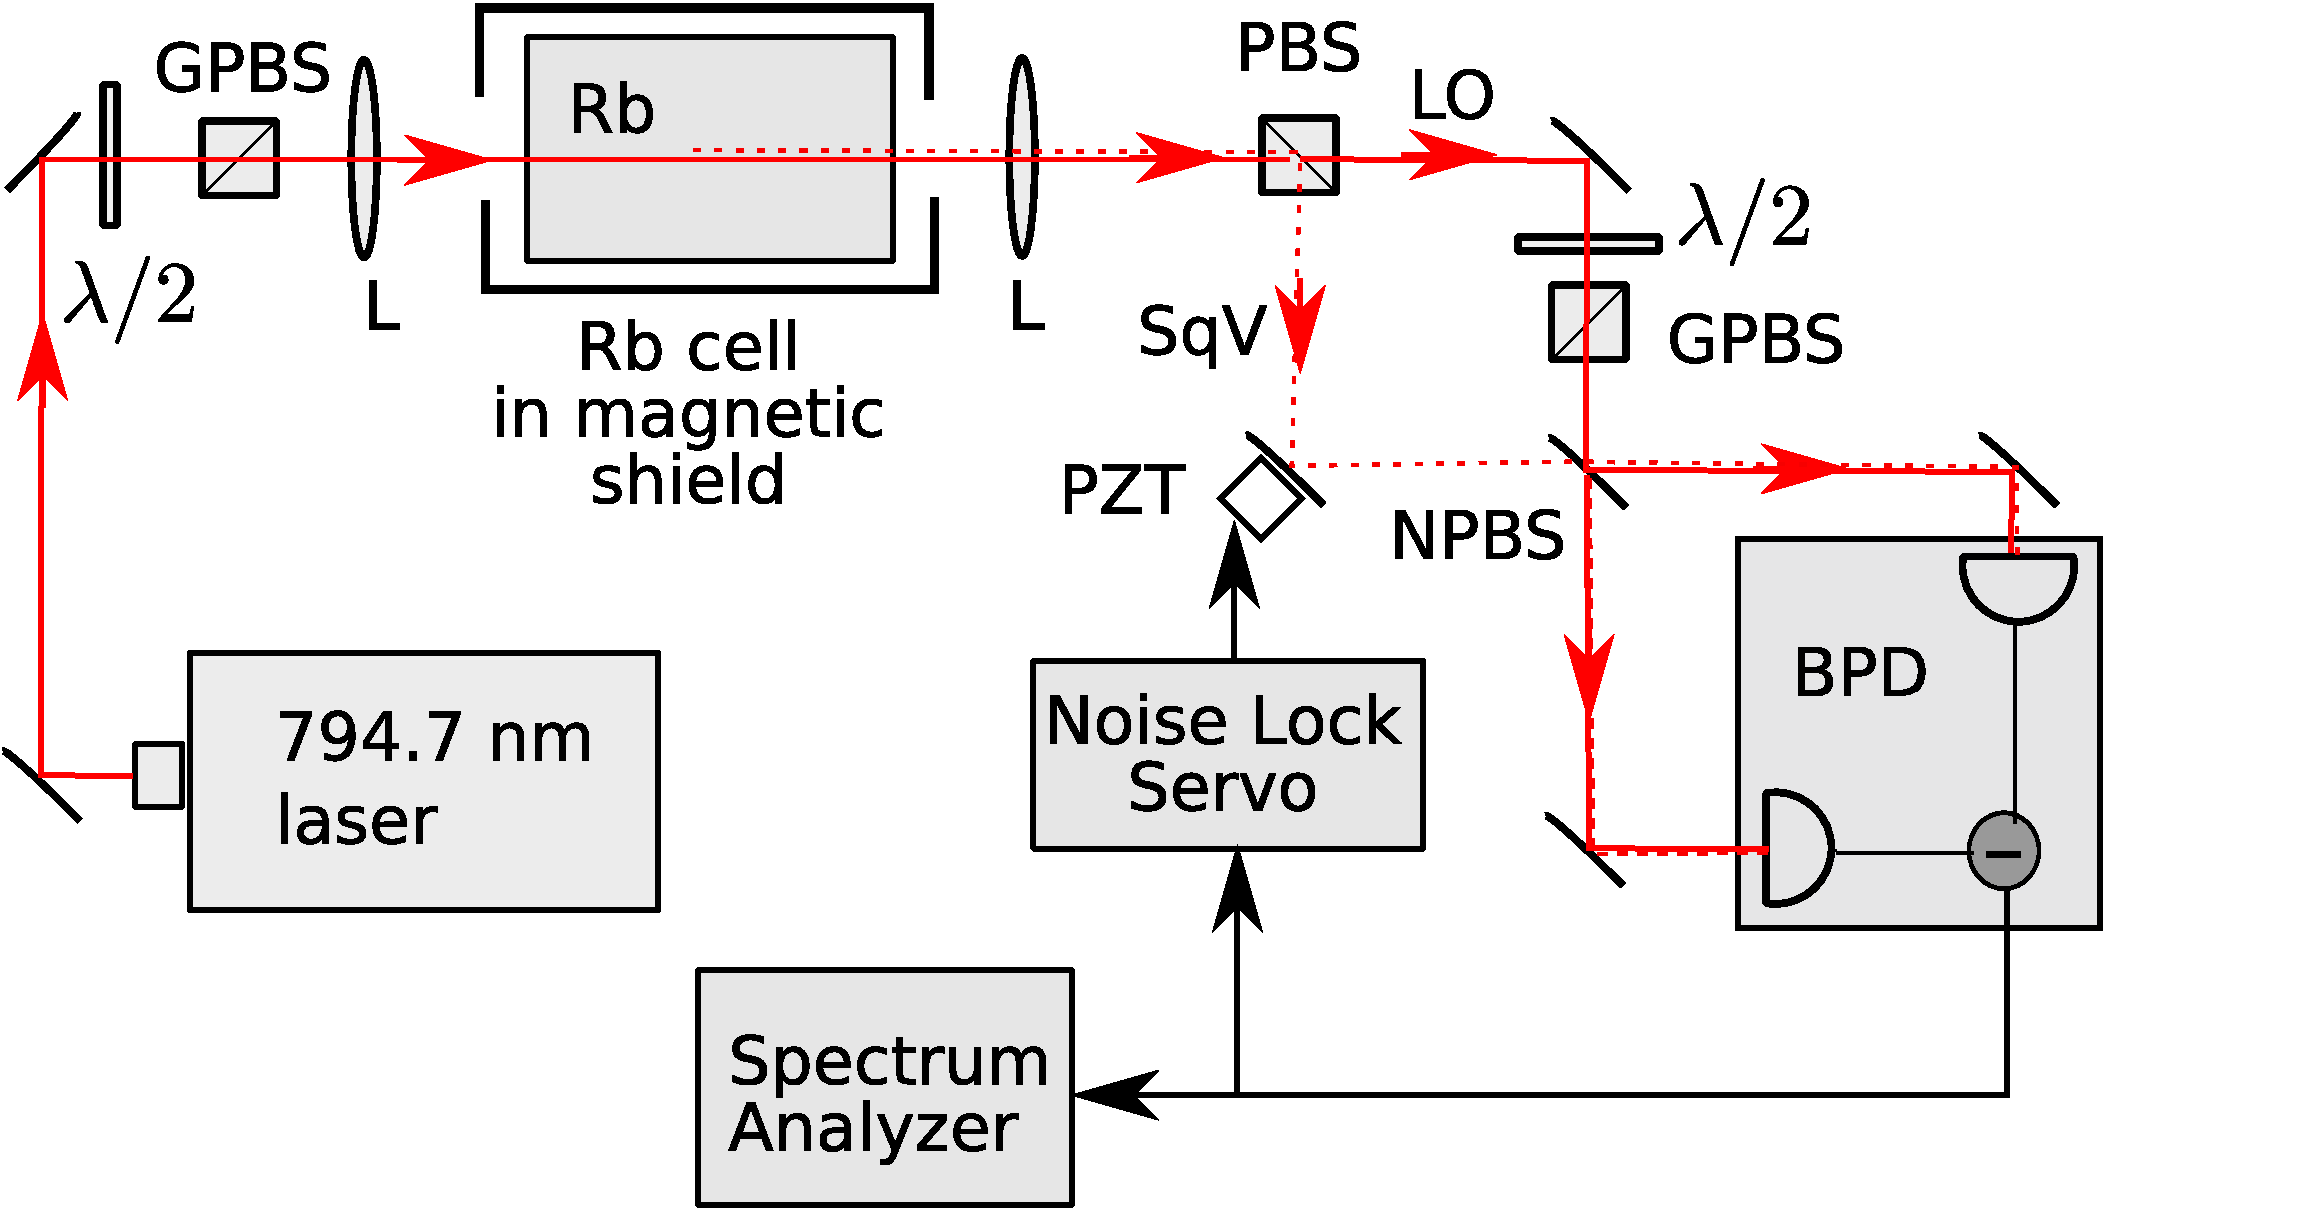
\includegraphics[width=1.0\columnwidth]{sr_setup.pdf}
        \caption{
                \label{fig:top_diagram} % spaces are big no-no withing labels
                % things like fig: are optional in the label but it helps
                % to orient yourself when you have multiple figures,
                % equations and tables
                {\bf Top structure for 3-stage pipeline.}
               I have six modules within my top module, corresponding to each of the pieces
               in this diagram: S1\_Reg, Reg\_File, S2\_Reg, Source\_Mux, Para\_ALU and S3\_Reg.
        }
\end{figure}

The hierarchy of my final design is shown in figure~\ref{fig:hierarchy}.
\begin{figure}[h] 
\centering
        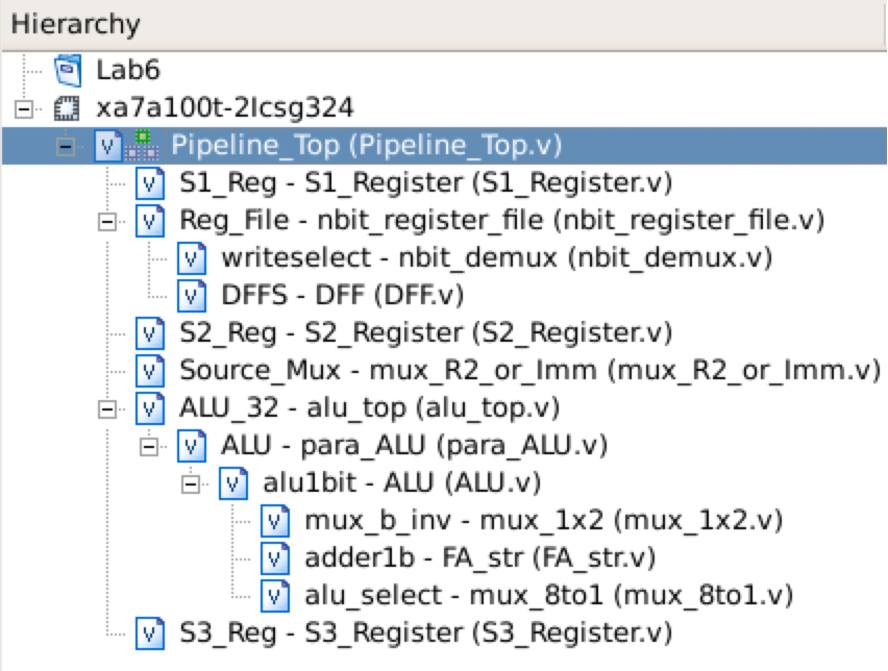
\includegraphics[width=0.7\columnwidth]{Hierarchy}

        \caption{
                \label{fig:hierarchy}
                {\bf Top module hierarchy.}
               The six modules inside my top module, along with all of their submodules.
        }
\end{figure}

\subsection{Pipeline Overview}

A 32-bit instruction very similar to MIPS instruction encoding is taken as an input to the stage one register module along with the clock (clk) and reset (rst) inputs. The instruction, labeled InstrIn, is parsed inside stage one as follows: InstrIn[31:30] can be ignored. If InstrIn[29] == 1 it is I-type, if InstrIn[29] == 0 it is R-type. InstrIn[28:26] is the 3-bit ALU op-code, InstrIn[25:21] is the destination register, InstrIn[20:16] is the first source register, InstrIn[15:11] is the second source register, and InstrIn[15:0] is the immediate field. Each of the three register stages will take new values at positive clock edges only. 

The values for the first and second source registers, labeled ReadSelect1 and ReadSelect2, respectively, are passed to the register file module called nbit\_register\_file, while all the other values
including Immediate, DataSource, AluOp, WriteSelect and WriteEnable, are passed to the stage two register module. 

Along with the outputs from stage one, stage two also takes as inputs the data read from the two source register locations, which is labeled ReadData1 and ReadData2. At the next positive clock edge all of the inputs of stage two are passed as outputs. ReadData1 is passed directly to the first input of a parameterized ALU sized to 32-bit, while ReadData2, Immediate and DataSource are all passed to a multiplexer. This multiplexer looks at the value of InstrIn[29] and decides whether to pass ReadData2 or Immediate to the second input of the ALU depending on whether it is R-type (0) or I-type (1). If the instruction is I-type, 16'd0 must be concatenated onto the front of the 16-bit immediate so that the ALU will get a 32-bit value. The ALU is combinational logic so it does not have to wait for a clock cycle. After it calculates an output based on its inputs and its opcode it passes the output to the stage three module. The remaining values, WriteSelect and WriteEnable, are passed directly to the stage three module. 

The stage three module is the simplest of the three, and doesn't do anything but receive values and pass them along at the next positive clock edge. AluOut is the final output, but it also gets passed to WriteData of the register file. WriteSelect and WriteEnable are also passed to the register file. This nbit\_register\_file module generates a 32 by 32-bit array of D flip flops to create the 32 registers. Finally, on the next positive clock edge WriteData is written to the register selected by WriteSelect. 

\section{Register File}

The first part of this lab to be tested was the nbit\_register\_file module. This was easy to do because a test bench for this module was already provided. The resulting simulation waveform for the register file using the provided test bench is shown in figure~\ref{fig:Filewaveform}. The only thing required to do here was to look at the sixteen instructions listed in the test bench and follow the simulation waveform to make sure everything matched up correctly. 

\begin{figure}[h] 
\centering
        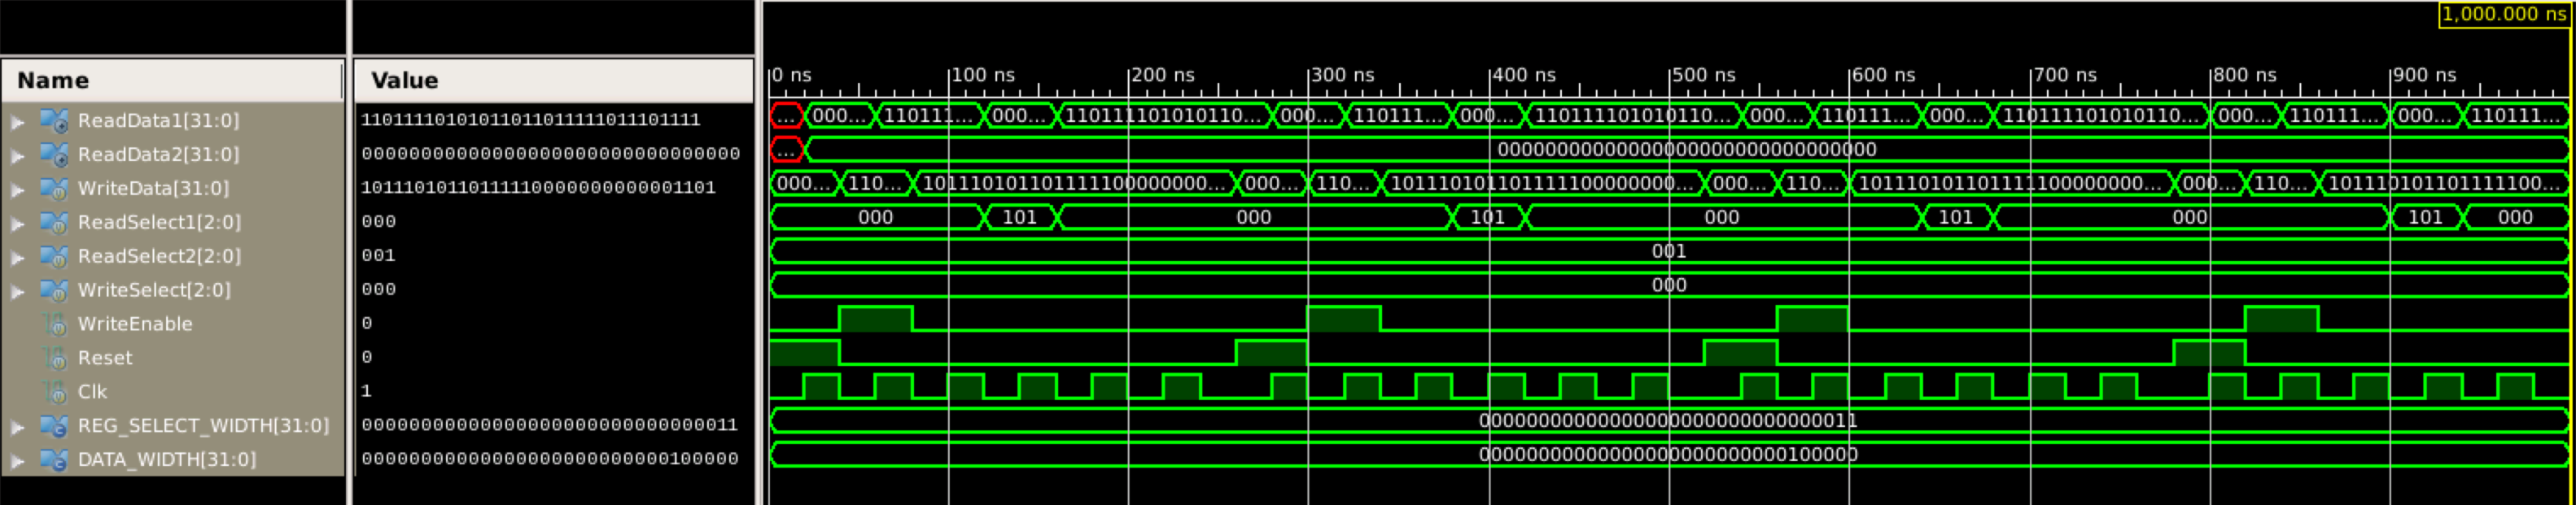
\includegraphics[width=1.0\columnwidth]{Reg_file_waveform}

        \caption{
                \label{fig:Filewaveform}
                {\bf nbit\_register\_file\_test waveform.}
               This image is also included separately.
        }
\end{figure}

\section{Bit-sliced ALU}

The next section that required resting was the ALU. This was also simple because we built the entire ALU in the previous lab. I copied every module from the previous lab into this project minus the registers and verification logic. After adding behavioral logic for the 6th opcode, SLT, I created a test bench with one to two test cases for each operation and followed the simulation waveform to confirm that I ended up with the correct results. The waveform for the ALU is shown in figure~\ref{fig:aluwaveform}.

\begin{figure}[h] 
\centering
        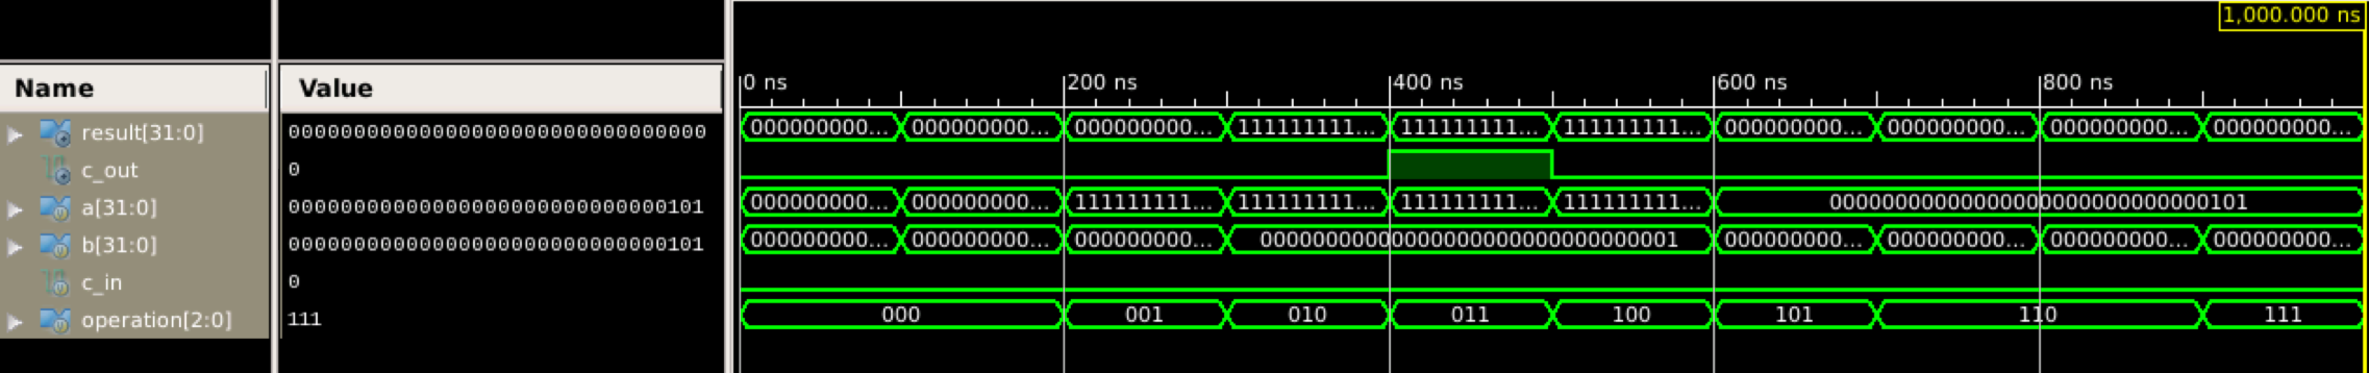
\includegraphics[width=1.0\columnwidth]{ALU_waveform}

        \caption{
                \label{fig:aluwaveform}
                {\bf alu\_top waveform.}
               This image is also included separately.
        }
\end{figure}



\section{Datapath}
I tested my final datapath design in two ways. First, I used the four sample instructions included in the lab procedure for my test bench. I checked the simulated waveform against the provided timing spreadsheet to make sure all of my values matched correctly. 

Next, I changed my instruction test bench to the provided list of thirteen instructions. These are the instructions that will be included in the test bench I submit. First off, I checked that the final output was correct. This is shown in figure~\ref{fig:finaloutput}. After confirming the final output, I started at the beginning and followed each instruction while also checking the individual registers R0-R31 by examining the values for the 32-bit wire w\_reg\_to\_outmux. All of the registers took the values I expected them to take. The final values for R0-R31 can be seen in figure~\ref{fig:regwaveform}.
\vspace{10 mm}

\begin{figure}[h] 
\centering
        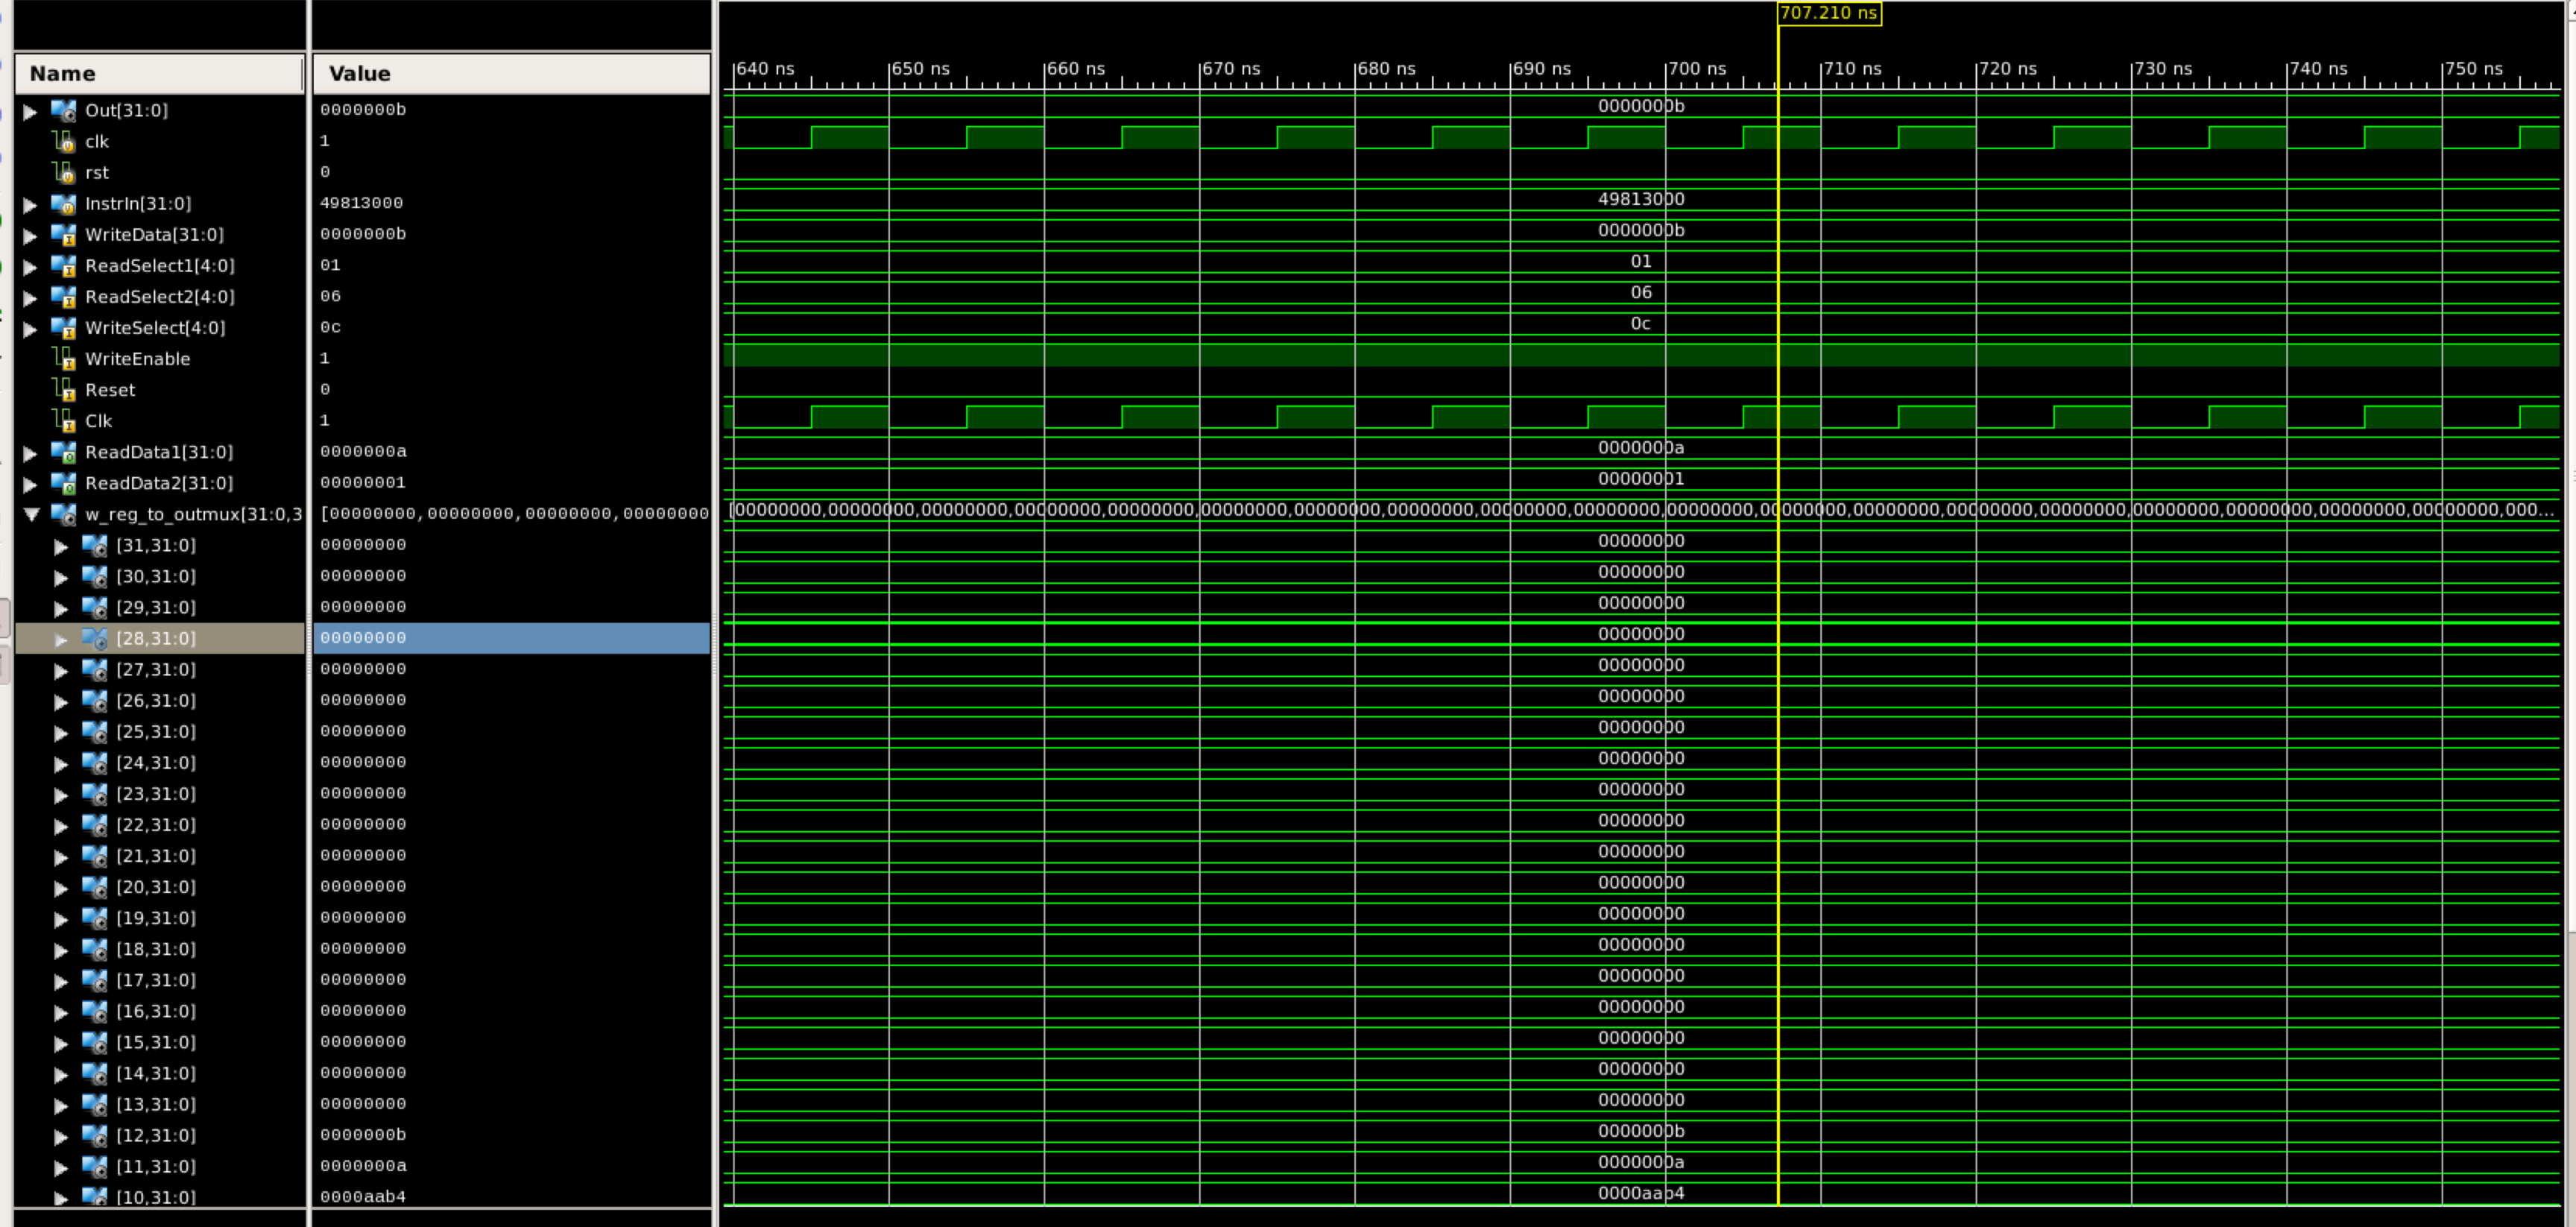
\includegraphics[width=1.0\columnwidth]{Final_output_waveform}

        \caption{
                \label{fig:finaloutput}
                {\bf Final output waveform.}
               This image is mainly used to show that the final output after all instructions have passed is 0x0B as expected.
        }
\end{figure}

\begin{figure}[ht] 
\centering
        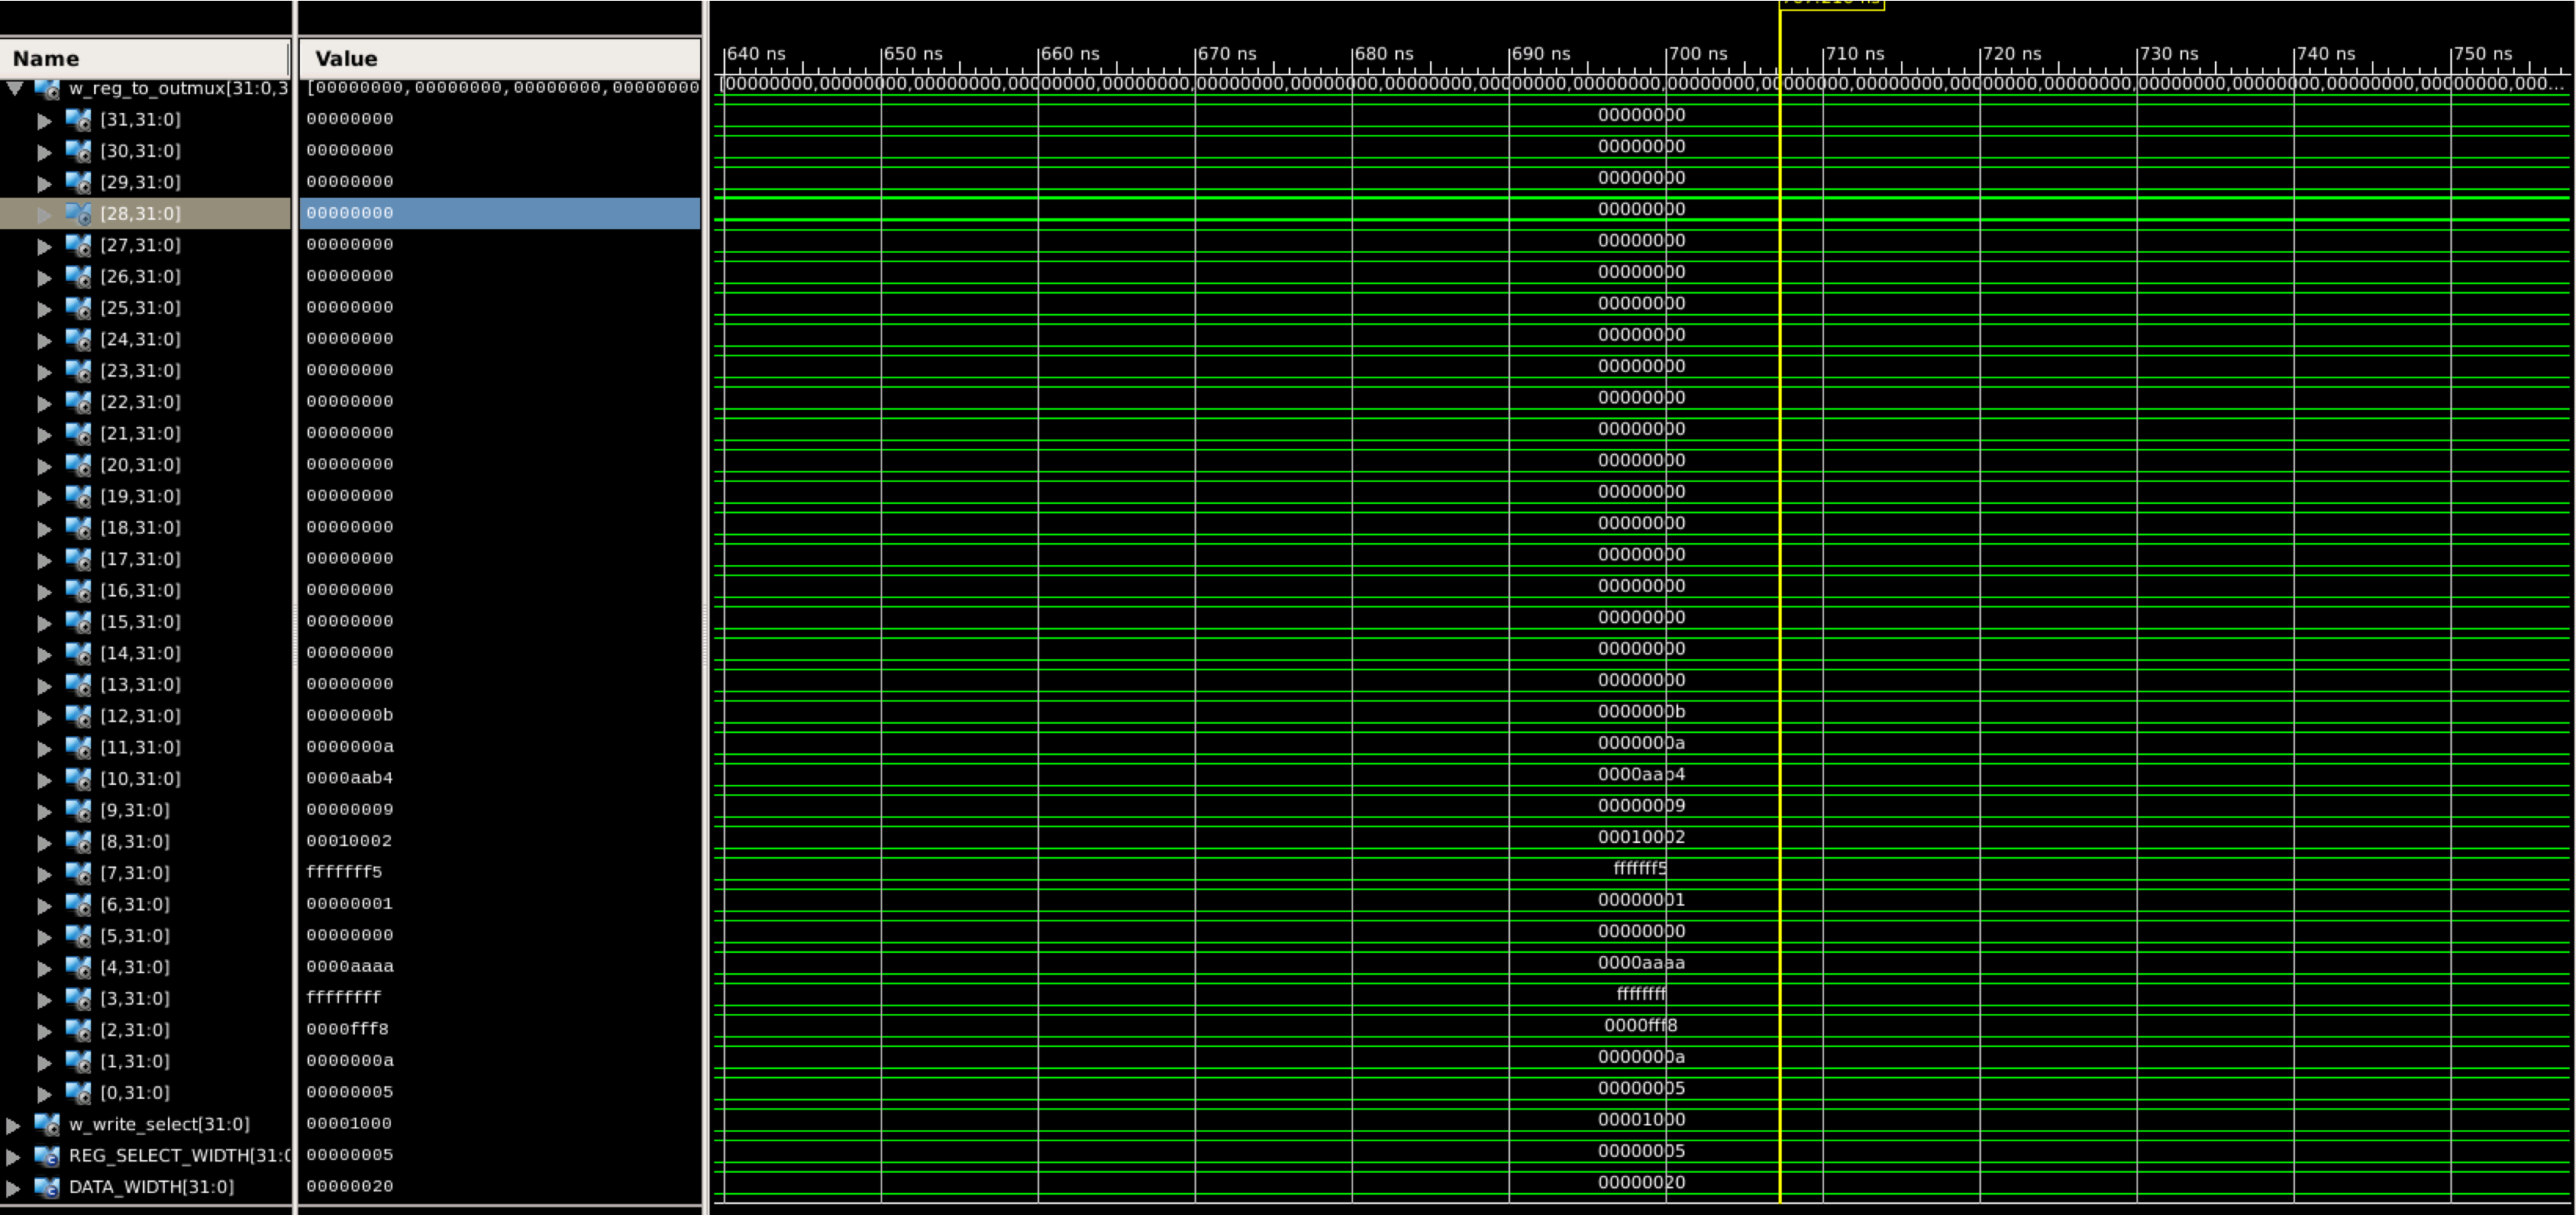
\includegraphics[width=1.0\columnwidth]{Final_reg_data_waveform}

        \caption{
                \label{fig:regwaveform}
                {\bf Final Register File Data.}
               The data within the registers R0-R31 can be seen by looking at the values of the outgoing wire array labeled w\_reg\_to\_outmux.
        }
\end{figure}


\section{Included Files}
\textbf{Source Files} \\
Pipeline\_Top.v \\
S1\_Register.v \\
nbit\_reg\_file.v \\
nbit\_demux.v \\
DFF.v \\
S2\_Register.v \\
mux\_R2\_or\_Imm.v \\
alu\_top.v \\
para\_alu.v \\
ALU.v \\
mux\_1x2.v \\
FA\_str.v \\
mux\_8to1.v \\
S3\_Register.v \\ \\
\textbf{Test Benches} \\
Pipeline\_Top\_tb.v \\
nbit\_register\_file\_test.v \\
alu\_top\_tb.v \\ \\
\textbf{Images} \\
pipeline\_pic.pdf \\
Hierarchy.pdf \\
Reg\_file\_waveform.pdf \\
ALU\_waveform.pdf \\
final\_output\_waveform.pdf \\
Final\_reg\_data\_waveform.pdf \\


\end{document}
